\section{Landslide}
\label{sec:landslide}

Motivated by the stress tests' inconsistency at finding concurrency bugs,
% TODO camready
we have built Landslide%\cite{landslide}
, a stateless model checker for \pebbles kernels and thread libraries.
Stateless model checking \cite{verisoft} offers an alternative
%concurrency testing approach
to stress testing,
in which the testing framework controls scheduling to force execution of a new thread interleaving in each iteration of a test.
It follows in the footsteps of related tools such as CHESS \cite{chess},
but also provides several important features for use in an educational setting,
such as heuristics to handle unusual student solutions, kernel-level testing, and user-friendly progress reports and HTML debugging traces.

\subsection{Design}

Conceptually,
Landslide is designed as follows.
Through several annotations in the kernel source, Landslide tracks
%the scheduler state to know
which threads are running or runnable.
(For testing thread libraries, these annotations are already provided in the reference kernel binary;
for testing kernels, the student must add them by hand.)
When execution reaches certain interesting {\em preemption points},
Landslide triggers artificial clock interrupts
to force the scheduler to run a different thread.
When a test finishes execution according
to one pattern of thread switches,
Landslide rewinds the simulation state
and resumes the test according to a different interleaving.
After each instruction,
Landslide applies several bug-detection predicates to
the program state to detect
illegal heap accesses,
deadlock, infinite loops, and panics.

{\bf Example.}
Figure \ref{fig:paradise}(a) shows an example concurrency bug. %which we will use as a running example.
The code implements a producer/consumer program, in which one thread sends work to the other through a shared list,
synchronized with a mutex and condition variable.
However, because the consumer code only checks once whether work exists before blocking,
%multiple
simultaneous consumers suffer
%as shown in Figure \ref{fig:paradise}(b),
a segfault when one receives a null \x{work} pointer. %and tries to dereference it

\definecolor{thread1}{RGB}{87,172,255}
\definecolor{thread2}{RGB}{255,201,102}
\definecolor{thread3}{RGB}{255,128,160}

\begin{figure}[t]
	\begin{tabular}{l|l}
	Consumer thread & Producer thread \\
	\hline
\begin{lstlisting}
mutex_lock(mx);
if (!work_exists())
  cond_wait(cvar,mx);
work = dequeue();
mutex_unlock(mx);
access(work->data);
\end{lstlisting}
	&
\begin{lstlisting}
mutex_lock(mx);

enqueue(work);
signal(cvar);

mutex_unlock(mx);
\end{lstlisting}
	\end{tabular}
	{\bf (a}) A buggy producer/consumer program, in which the consumer thread only checks \x{work_exists()} once.
	\vspace{1em}
	\\
	%%%%%%%%%%%%%%%%%%%%%%%%%%%%%%%%%%%%%%%%
%	\begin{tabular}{l|l|l}
%	\cellcolor{thread1} {\bf Thread 1} & \cellcolor{thread2} {\bf Thread 2} & \cellcolor{thread3} {\bf Thread 3} \\
%	\hline
%\begin{lstlisting}
%lock();
%if (!work())
%  wait();
%\end{lstlisting}
%& & \\
%&
%\begin{lstlisting}
%lock();
%enqueue();
%signal();
%unlock();
%\end{lstlisting}
%& \\
%& &
%\begin{lstlisting}
%lock();
%dequeue();
%unlock();
%\end{lstlisting}
%\\
%\begin{lstlisting}
%dequeue();
%unlock();
%// SIGSEGV
%\end{lstlisting}
%& &
%	\begin{center}
%	{\bf (b)} Interleaving with two consumer threads. The second bypasses \x{cond_wait()}, causing the first to receive \x{NULL}. %in which one receives \x{NULL}.
	%%%%%%%%%%%%%%%%%%%%%%%%%%%%%%%%%%%%%%%%
	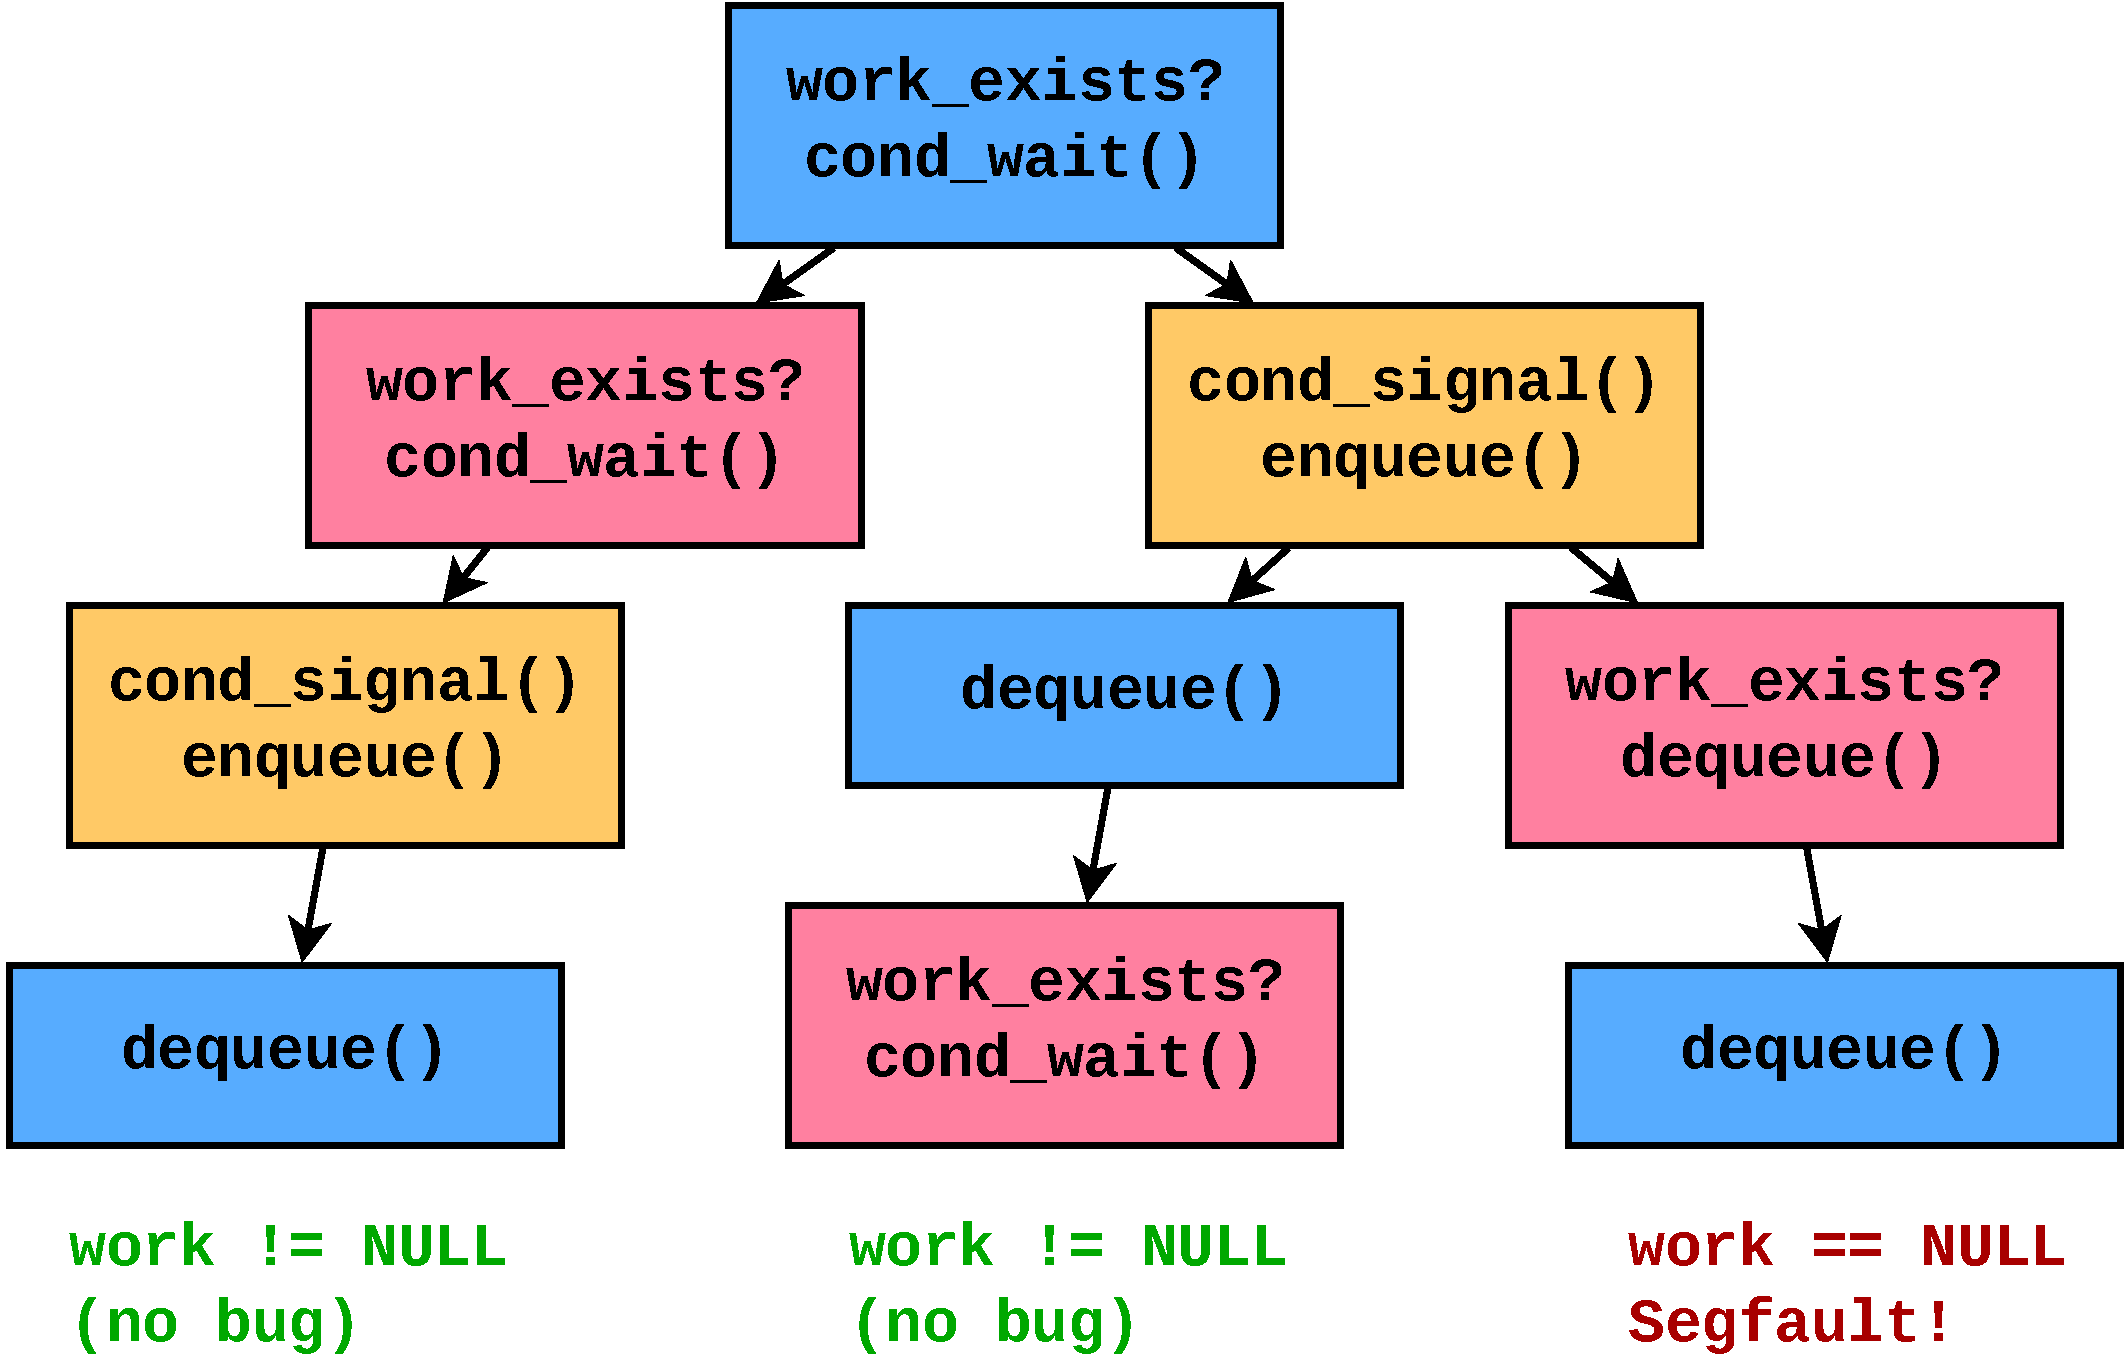
\includegraphics[width=0.48\textwidth]{execution-tree.pdf}
	{\bf (b)} The state space of all interleavings forms an execution tree. %The interleaving in (b) is the rightmost branch.
	The bug is observed when the second consumer thread bypasses \x{cond_wait()}, causing the first to receive \x{NULL}.
	%%%%%%%%%%%%%%%%%%%%%%%%%%%%%%%%%%%%%%%%
	\caption{Example concurrency bug.}
	\label{fig:paradise}
\end{figure}

{\bf State space exploration.}
To trigger the interleaving which exposes this bug, threads must be preempted at the boundaries of the synchronization primitives (either when \x{cond_wait} blocks or at the end of \x{mutex_unlock}).
Landslide automatically considers these boundaries to be {\em preemption points}: candidate sites for timer-driven thread switches.
It can also add preemption points dynamically,
as identified by an integrated data-race analysis \cite{tsan,fasttrack},
to expose shared-memory bugs when synchronization is absent.

The branching possibilities arising from each preemption point produce an execution tree, or state space,
as shown in Figure \ref{fig:paradise}(b).
%As these state spaces are exponentially-sized,
Landslide uses Dynamic Partial Order Reduction (DPOR) \cite{dpor} to identify and prune equivalent interleavings
to mitigate the exponential explosion of these state spaces.
% TODO make sure this gets mentioned later, if not here
%and state space estimation \cite{estimation} to predict which
% TODO CAMREADY: cite oopsla
% In principle, the combination of synchronization API and data-race preemption points is sufficient to expose all bugs that are reachable by any combination of timer interrupts on any instructions.
This reduction requires only tracing the memory accesses of each thread,
so we are able to perform it behind-the-scenes, without consuming any student attention.

\subsection{Identifying Bugs}

Landslide checks for bugs in several ways.
It can identify assertion failures, use-after-free and other invalid heap accesses, and
deadlocks, and also includes a heuristic check for infinite loops and livelock.
%Note that our use of the term ``race condition'' throughout this paper refers to concurrency errors in general, a category that includes data races, atomicity violations, and nondeterministic deadlocks.
%In contrast with analyses that directly detect data races~\cite{tsan},
Although Landslide employs a data-race analysis to decide where to preempt,
it does not directly classify suspicious memory accesses as bugs,
but rather seeks concrete, observable failures that can arise from many different types of errors.

When Landslide identifies a bug, it outputs an HTML-formatted
{\em preemption trace}.
Figure~\ref{fig:trace} shows a typical output for the example bug in Figure \ref{fig:paradise}.
The trace reports what kind of bug was detected
and each preemption point in the current interleaving:
which thread was running, a trace of its stack when it was preempted, and the thread that ran next.
Hence, students can bypass tediously reconstructing the schedule using \x{printf},
and hopefully better understand the concurrent execution that exposed the bug,

\newcommand\hilight[2]{\color{#1}#2\color{black}\xspace}
\definecolor{orange}{RGB}{192,96,0}
\definecolor{olivegreen}{RGB}{0,127,0}
\definecolor{brickred}{RGB}{192,0,0}
\definecolor{commentblue}{RGB}{0,0,192}

\begin{figure*}[t]
	\hilight{brickred}{{\bf TID 4 was killed by a page fault! (Faulting eip: 0x1000294; addr: 0x00000000)}} (53 interleavings tested)
	\\
	\begin{tabular}{|l|l|l|}
		\hline
		\multicolumn{1}{|c|}{\bf TID 4} &
		\multicolumn{1}{c|}{\bf TID 5} &
		\multicolumn{1}{c|}{\bf TID 6} \\
		\hline
		\hline
		0x010003d5 \hilight{olivegreen}{\x{deschedule}} (syscalls.c:7) & & \\
		0x010011a4 \hilight{olivegreen}{\x{cond_wait}} (cond.c:21) & & \\
		0x010001e0 \hilight{olivegreen}{\x{consumer}} (main.c:30) & & \\
		0x01000259 \hilight{olivegreen}{\x{child_thread}} (main.c:42) & & \\
		\hline
		& 0x010034f5 \hilight{olivegreen}{\x{mutex_unlock}} (mutex.c:19) & \\
		& 0x01000037 \hilight{olivegreen}{\x{producer}} (main.c:74) & \\
		& 0x01000100 \hilight{olivegreen}{\x{main}} (main.c:88) & \\
		\hline
		& & 0x010034f5 \hilight{olivegreen}{\x{mutex_unlock}} (mutex.c:19) \\
		& & 0x0100020a \hilight{olivegreen}{\x{consumer}} (main.c:33) \\
		& & 0x01000259 \hilight{olivegreen}{\x{child_thread}} (main.c:42) \\
		\hline
		0x01000294 \hilight{olivegreen}{\x{access}} (main.c:17) & & \\
		0x01000216 \hilight{olivegreen}{\x{consumer}} (main.c:34) & & \\
		0x01000259 \hilight{olivegreen}{\x{child_thread}} (main.c:42) & & \\
		\hline
	\end{tabular}
	\caption{Example preemption trace provided by Landslide as debugging output for the bug in Figure~\ref{fig:paradise}.}
	\label{fig:trace}
\end{figure*}

\subsection{Instrumentation}

For the thread library project, Landslide instruments student implementations automatically.
We provide a custom reference kernel binary equipped with the kernel instrumentations (described below)
so Landslide can track threads' lifecycles. %the lifecycle of threads.
The userspace \x{malloc} and \x{assert} are also provided in the basecode, and tracked similarly.
Landslide's data-race analysis must understand the locking discipline,
so it searches the student's code for functions named \x{mutex_lock} and \x{mutex_unlock} (as mandated by the assignment handout),
and assumes they at least provide mutual exclusion\footnote{
	To relax this assumption, we provide a special test case for mutexes,
	in which Landslide may preempt and search for data races in the mutex implementation itself.
}.
All other thread library components are treated as unknown, and subject to preemption anywhere.

To test \pebbles kernels directly, they must be annotated to inform Landslide of certain important concurrency events.
Because the kernel project leaves internal code structure as an open-ended design decision,
Landslide cannot search for specific function names. % like it does for P2s.
Instead, we provide a set of functions named with the prefix \x{tell_landslide}
to denote when a thread runs \x{fork}, \x{sleep}, or \x{vanish}, when a thread is added to or removed from the runqueue, and when a thread becomes blocked on a mutex.
Users must also list all core scheduler, context switch, and timer handling routines, so Landslide can ignore their memory accesses for the sake of DPOR
(otherwise, threads would always conflict with each other and DPOR would achieve no reduction).

\subsection{Heuristics}

Student submissions may behave in extraordinary ways which violate the assumptions of many modern model checkers.
Landslide refuses to test code which fails the hurdle criteria (\sect{\ref{sec:grading}}),
but it must support testing any legal, yet distasteful, solution.
%Hence, we added several heuristic
For example, students may use open-coded \x{yield} or \x{xchg} loops rather than the mutex abstraction. %(though it is discouraged).
To avoid getting stuck in a cyclic (infinite) state space, Landslide keeps a ``yield loop'' counter for each thread;
when a thread \x{yield}s 10 times without otherwise making progress, Landslide marks it blocked.
%
In extreme cases, this may erroneously seem like deadlock when all threads \x{yield} many times coincidentally.
To avoid wasting student time with false alarms, % the ultimate sin
Landslide will reset all blocked threads' yield-loop counters,
retrying potentially up to 128 times before reporting a true deadlock.

Students may also break abstraction by open-coding a \x{mutex_unlock} sequence.
Landslide must track lock operations for accurate data-race analysis,
so to catch these patterns, it
%learns the size of the \x{mutex} struct, then
checks accesses against stored lock addresses blocked on by other threads.
Similarly, these rogue unlock accesses may unblock a yield-looping thread.
